\documentclass[14pt,dvipdfmx,uplatex]{beamer}
\usetheme{Madrid} 
\setbeamertemplate{footline}[page number]{}
\beamertemplatenavigationsymbolsempty
\usepackage{mypresentation}
%\AtBeginShipoutFirst{\special{pdf:tounicode EUC-UCS2}}
\usepackage{shapepar}
\usepackage{tikz}
\usetikzlibrary{arrows}
\usetikzlibrary{shapes.callouts}
\usetikzlibrary{decorations.pathmorphing}
\usetikzlibrary{positioning}

\usepackage[noalphabet]{pxchfon}
\definecolor{ikkonzome}{rgb}	{	0.9961	,	0.7569	,	0.7373	}
\definecolor{ishitake}{rgb}	{	0.9961	,	0.6941	,	0.7059	}
\definecolor{momo}{rgb}	        {	0.9961	,	0.6824	,	0.8039	}
\definecolor{kobai}{rgb}	{	0.9412	,	0.4235	,	0.5569	}
\definecolor{nakabeni}{rgb}	{	0.9451	,	0.2706	,	0.4941	}
\definecolor{sakura}{rgb}	{	0.9333	,	0.8353	,	0.8353	}
\definecolor{arazome}{rgb}	{	0.9725	,	0.7216	,	0.7843	}
\definecolor{usubeni}{rgb}	{	0.8471	,	0.4471	,	0.5451	}
\definecolor{hisame}{rgb}	{	0.7451	,	0.4039	,	0.4039	}
\definecolor{toki}{rgb}	        {	0.9569	,	0.6431	,	0.6353	}
\definecolor{sakuranezumi}{rgb}	{	0.6941	,	0.6039	,	0.6078	}
\definecolor{sango}	{rgb}	{	0.8471	,	0.4157	,	0.3725	}
\definecolor{akane}	{rgb}	{	0.7529	,	0.0118	,	0.3451	}
\definecolor{choshun}{rgb}	{	0.7490	,	0.5255	,	0.5255	}
\definecolor{karakurenai}{rgb}	{	0.7373	,	0.0118	,	0.2667	}
\definecolor{enji}{rgb}	        {	0.6275	,	0.0863	,	0.3176	}
\definecolor{keshiaka}{rgb}	{	0.6275	,	0.4275	,	0.4275	}
\definecolor{kokiake}{rgb}	{	0.5059	,	0.0706	,	0.2549	}
\definecolor{jinzamomi}{rgb}	{	0.9098	,	0.4549	,	0.4157	}
\definecolor{mizugaki}{rgb}	{	0.7294	,	0.5529	,	0.4784	}
\definecolor{umenezumi}{rgb}	{	0.5882	,	0.3922	,	0.3882	}
\definecolor{suoko}{rgb}        {	0.5843	,	0.2667	,	0.2431	}
\definecolor{akabeni}{rgb}	{	0.8039	,	0.0784	,	0.3725	}
\definecolor{shinshu}{rgb}	{	0.6431	,	0.0353	,	0.0000	}
\definecolor{azuki}{rgb}	{	0.5255	,	0.0235	,	0.0000	}
\definecolor{ginshu}{rgb}	{	0.7490	,	0.2824	,	0.0588	}
\definecolor{ebicha}{rgb}	{	0.4549	,	0.2706	,	0.2627	}
\definecolor{kuriume}{rgb}	{	0.5843	,	0.3804	,	0.4314	}
\definecolor{akebono}{rgb}	{	0.8902	,	0.5961	,	0.4941	}
\definecolor{hanezu}{rgb}	{	0.7882	,	0.5961	,	0.5373	}
\definecolor{sangoshu}{rgb}	{	0.8196	,	0.5059	,	0.4471	}
\definecolor{shozyohi}{rgb}	{	0.7686	,	0.0000	,	0.0000	}
\definecolor{shikancha}{rgb}	{	0.5569	,	0.3294	,	0.1882	}
\definecolor{kakishibu}{rgb}	{	0.6745	,	0.4078	,	0.3333	}
\definecolor{benikaba}{rgb}	{	0.7137	,	0.3373	,	0.2941	}
\definecolor{benitobi}{rgb}	{	0.6196	,	0.3176	,	0.2706	}
\definecolor{benihihada}{rgb}	{	0.5020	,	0.3137	,	0.2353	}
\definecolor{kurotobi}{rgb}	{	0.3176	,	0.2000	,	0.1490	}
\definecolor{benihi}{rgb}	{	0.8235	,	0.4745	,	0.1922	}
\definecolor{terigaki}{rgb}	{	0.8118	,	0.4627	,	0.1804	}
\definecolor{ake}{rgb}	        {	0.7804	,	0.3098	,	0.1725	}
\definecolor{edocha}{rgb}	{	0.6863	,	0.4353	,	0.2941	}
\definecolor{bengara}{rgb}	{	0.6392	,	0.1569	,	0.0196	}
\definecolor{hihada}{rgb}	{	0.5412	,	0.3412	,	0.2353	}
\definecolor{shishi}{rgb}	{	0.8549	,	0.6863	,	0.5961	}
\definecolor{araishu}{rgb}	{	0.9294	,	0.4902	,	0.4549	}
\definecolor{akago}{rgb}	{	0.8118	,	0.5765	,	0.4275	}
\definecolor{tokigaracha}{rgb}	{	0.7922	,	0.5255	,	0.3686	}
\definecolor{otan}{rgb}	        {	0.8157	,	0.4157	,	0.2235	}
\definecolor{komugi}{rgb}	{	0.8157	,	0.6549	,	0.5098	}
\definecolor{rakuda}{rgb}	{	0.6784	,	0.5255	,	0.4118	}
\definecolor{tsurubami}{rgb}	{	0.6275	,	0.4392	,	0.3961	}
\definecolor{ama}{rgb}	        {	0.7765	,	0.6902	,	0.5843	}
\definecolor{nikkei}{rgb}	{	0.7216	,	0.4667	,	0.3725	}
\definecolor{renga}{rgb}	{	0.6902	,	0.3765	,	0.3098	}
\definecolor{sohi}{rgb}   	{	0.8078	,	0.5098	,	0.2078	}
\definecolor{enshucha}{rgb}	{	0.6706	,	0.4275	,	0.1608	}
\definecolor{karacha}{rgb}	{	0.5765	,	0.4235	,	0.1490	}
\definecolor{kabacha}{rgb}	{	0.6353	,	0.3725	,	0.1569	}
\definecolor{sodenkaracha}{rgb}	{	0.5216	,	0.3490	,	0.1373	}
\definecolor{suzumecha}{rgb}	{	0.4745	,	0.3176	,	0.1255	}
\definecolor{kurikawacha}{rgb}	{	0.4078	,	0.2745	,	0.1098	}
\definecolor{momoshiocha}{rgb}	{	0.3490	,	0.2353	,	0.0902	}
\definecolor{tobi}{rgb}	        {	0.4353	,	0.3098	,	0.1412	}
\definecolor{kurumizome}{rgb}	{	0.6667	,	0.5333	,	0.3333	}
\definecolor{kaba}{rgb}	        {	0.8196	,	0.4588	,	0.1294	}
\definecolor{korosen}{rgb}	{	0.5059	,	0.3843	,	0.1608	}
\definecolor{kogecha}{rgb}	{	0.3333	,	0.2549	,	0.1098	}
\definecolor{kokikuchinashi}{rgb}	{	0.8078	,	0.5922	,	0.3490	}
\definecolor{araigaki}{rgb}	{	0.8157	,	0.5529	,	0.3176	}
\definecolor{taisha}{rgb}	{	0.6353	,	0.4196	,	0.2078	}
\definecolor{akashirotsurubami}{rgb}	{	0.8078	,	0.6118	,	0.4157	}
\definecolor{tonocha}{rgb}	{	0.5922	,	0.4039	,	0.2000	}
\definecolor{sencha}{rgb}	{	0.5255	,	0.3529	,	0.1490	}
\definecolor{sharegaki}{rgb}	{	0.8549	,	0.7098	,	0.4863	}
\definecolor{ko}{rgb}	        {	0.9529	,	0.8275	,	0.6627	}
\definecolor{usugaki}{rgb}	{	0.8627	,	0.7294	,	0.5294	}
\definecolor{koji}{rgb}	        {	0.8275	,	0.6039	,	0.2706	}
\definecolor{umezome}{rgb}	{	0.8667	,	0.7373	,	0.4235	}
\definecolor{beniukon}{rgb}	{	0.8549	,	0.5843	,	0.2549	}
\definecolor{chojicha}{rgb}	{	0.5569	,	0.4000	,	0.1098	}
\definecolor{kenpozome}{rgb}	{	0.3059	,	0.2667	,	0.0627	}
\definecolor{biwacha}{rgb}	{	0.7333	,	0.5294	,	0.1922	}
\definecolor{kohaku}{rgb}	{	0.8039	,	0.5961	,	0.2471	}
\definecolor{usuko}{rgb}	{	0.8745	,	0.7373	,	0.4824	}
\definecolor{kuchiba}{rgb}	{	0.8157	,	0.6157	,	0.3216	}
\definecolor{kincha}{rgb}	{	0.7725	,	0.4902	,	0.2000	}
\definecolor{chozizome}{rgb}	{	0.5686	,	0.3961	,	0.1608	}
\definecolor{kitsune}{rgb}	{	0.6392	,	0.4431	,	0.1804	}
\definecolor{hushizome}{rgb}	{	0.5804	,	0.4353	,	0.1608	}
\definecolor{kyara}{rgb}	{	0.4510	,	0.3373	,	0.1255	}
\definecolor{susutake}{rgb}	{	0.4588	,	0.3529	,	0.1176	}
\definecolor{shirocha}{rgb}	{	0.7529	,	0.6588	,	0.4118	}
\definecolor{odo}{rgb}	        {	0.7137	,	0.6039	,	0.3137	}
\definecolor{ginsusutake}{rgb}	{	0.5608	,	0.4745	,	0.2392	}
\definecolor{kigaracha}{rgb}	{	0.7490	,	0.6196	,	0.2745	}
\definecolor{kobicha}	{rgb}	{	0.5020	,	0.4118	,	0.1765	}
\definecolor{usuki}	{rgb}	{	0.8549	,	0.7804	,	0.4275	}
\definecolor{yamabuki}	{rgb}	{	0.9098	,	0.8000	,	0.2039	}
\definecolor{tamago}	{rgb}	{	0.8275	,	0.7412	,	0.3373	}
\definecolor{hajizome}	{rgb}	{	0.7412	,	0.6039	,	0.2431	}
\definecolor{yamabukicha}{rgb}	{	0.7059	,	0.5765	,	0.2275	}
\definecolor{kuwazome}	{rgb}	{	0.6471	,	0.5255	,	0.2118	}
\definecolor{namakabe}	{rgb}	{	0.5569	,	0.4549	,	0.1843	}
\definecolor{kuchinashi}{rgb}	{	0.8078	,	0.7333	,	0.3843	}
\definecolor{tomorokoshi}{rgb}	{	0.7804	,	0.7020	,	0.2941	}
\definecolor{shirotsurubami}{rgb}	{	0.8745	,	0.8235	,	0.5922	}
\definecolor{kitsurubami}{rgb}	{	0.6863	,	0.6039	,	0.2118	}
\definecolor{toou}	{rgb}	{	0.8353	,	0.7725	,	0.4235	}
\definecolor{hanaba}	{rgb}	{	0.8549	,	0.8000	,	0.4941	}
\definecolor{torinoko}	{rgb}	{	0.8431	,	0.8118	,	0.6902	}
\definecolor{ukon}	{rgb}	{	0.8039	,	0.7216	,	0.3059	}
\definecolor{kikuchiba}	{rgb}	{	0.7765	,	0.6667	,	0.2902	}
\definecolor{rikyushiracha}{rgb}{	0.6627	,	0.6471	,	0.4784	}
\definecolor{rikyucha}	{rgb}	{	0.5176	,	0.5176	,	0.2588	}
\definecolor{aku}	{rgb}	{	0.5294	,	0.5059	,	0.4039	}
\definecolor{higosusutake}{rgb}	{	0.4863	,	0.4510	,	0.3059	}
\definecolor{rokocha}	{rgb}	{	0.4157	,	0.4353	,	0.3686	}
\definecolor{mirucha}	{rgb}	{	0.4471	,	0.4471	,	0.3725	}
\definecolor{natane}	{rgb}	{	0.7216	,	0.6863	,	0.3882	}
\definecolor{kimirucha}	{rgb}	{	0.5373	,	0.5059	,	0.2549	}
\definecolor{uguisucha}	{rgb}	{	0.4118	,	0.3882	,	0.1961	}
\definecolor{nanohana}	{rgb}	{	0.9882	,	0.9882	,	0.3804	}
\definecolor{kariyasu}	{rgb}	{	0.8039	,	0.7686	,	0.3882	}
\definecolor{kihada}	{rgb}	{	0.9608	,	0.9137	,	0.2863	}
\definecolor{zoge}	{rgb}	{	0.8863	,	0.8235	,	0.7216	}
\definecolor{wara}	{rgb}	{	0.7882	,	0.7490	,	0.4706	}
\definecolor{macha}	{rgb}	{	0.6235	,	0.6392	,	0.4863	}
\definecolor{yamabato}	{rgb}	{	0.5137	,	0.5176	,	0.4000	}
\definecolor{mushikuri}	{rgb}	{	0.8196	,	0.8000	,	0.6118	}
\definecolor{aokuchiba}	{rgb}	{	0.6275	,	0.6392	,	0.3451	}
\definecolor{hiwacha}	{rgb}	{	0.6784	,	0.6863	,	0.4196	}
\definecolor{ominaeshi}	{rgb}	{	0.8745	,	0.8863	,	0.4039	}
\definecolor{wasabi}	{rgb}	{	0.5922	,	0.6824	,	0.5765	}
\definecolor{uguisu}	{rgb}	{	0.3333	,	0.4118	,	0.0627	}
\definecolor{hiwa}	{rgb}	{	0.7098	,	0.7216	,	0.2392	}
\definecolor{aoshirotsurubami}{rgb}	{	0.5961	,	0.6471	,	0.4471	}
\definecolor{yanagicha}	{rgb}	{	0.5373	,	0.5725	,	0.3529	}
\definecolor{rikancha}	{rgb}	{	0.3333	,	0.4196	,	0.2863	}
\definecolor{aikobicha}	{rgb}	{	0.2706	,	0.3412	,	0.2353	}
\definecolor{koke}	{rgb}	{	0.4941	,	0.5686	,	0.3922	}
\definecolor{miru}	{rgb}	{	0.1529	,	0.3216	,	0.1843	}
\definecolor{sensai}	{rgb}	{	0.1373	,	0.2863	,	0.1608	}
\definecolor{baiko}	{rgb}	{	0.5529	,	0.6157	,	0.3922	}
\definecolor{iwai}	{rgb}	{	0.3059	,	0.4118	,	0.2784	}
\definecolor{hiwamoegi}	{rgb}	{	0.4431	,	0.6824	,	0.2431	}
\definecolor{yanagisusutake}{rgb}	{	0.2039	,	0.3333	,	0.1255	}
\definecolor{urayanagi}	{rgb}	{	0.5843	,	0.6824	,	0.2431	}
\definecolor{usumoegi}	{rgb}	{	0.4824	,	0.6706	,	0.2275	}
\definecolor{yanagizome}{rgb}	{	0.4353	,	0.6000	,	0.2078	}
\definecolor{moegi}	{rgb}	{	0.3020	,	0.5961	,	0.1882	}
\definecolor{aoni}	{rgb}	{	0.1216	,	0.4196	,	0.2431	}
\definecolor{matsuba}	{rgb}	{	0.1098	,	0.3686	,	0.2118	}
\definecolor{usuao}	{rgb}	{	0.5529	,	0.7059	,	0.6118	}
\definecolor{wakatake}	{rgb}	{	0.3843	,	0.6824	,	0.5059	}
\definecolor{yanaginezumi}{rgb}	{	0.5020	,	0.6078	,	0.5490	}
\definecolor{oitake}	{rgb}	{	0.4157	,	0.5412	,	0.4392	}
\definecolor{sensaimidori}{rgb}	{	0.2549	,	0.3882	,	0.2627	}
\definecolor{midori}	{rgb}	{	0.0000	,	0.4824	,	0.0000	}
\definecolor{byakuroku}	{rgb}	{	0.6078	,	0.7333	,	0.6196	}
\definecolor{sabiseiji}	{rgb}	{	0.5333	,	0.6588	,	0.5804	}
\definecolor{rokusho}	{rgb}	{	0.3373	,	0.6039	,	0.4039	}
\definecolor{tokusa}	{rgb}	{	0.2549	,	0.4706	,	0.3922	}
\definecolor{onandocha}	{rgb}	{	0.2039	,	0.3725	,	0.3098	}
\definecolor{aotake}	{rgb}	{	0.1412	,	0.5176	,	0.4353	}
\definecolor{rikyunezumi}{rgb}	{	0.4157	,	0.5686	,	0.5490	}
\definecolor{birodo}	{rgb}	{	0.1059	,	0.4275	,	0.3608	}
\definecolor{mishiao}	{rgb}	{	0.1098	,	0.4588	,	0.3882	}
\definecolor{aimirucha}	{rgb}	{	0.2510	,	0.4000	,	0.3608	}
\definecolor{tonotya}	{rgb}	{	0.3059	,	0.4941	,	0.4392	}
\definecolor{mizuasagi}	{rgb}	{	0.1569	,	0.6745	,	0.6745	}
\definecolor{seji}	{rgb}	{	0.4745	,	0.6588	,	0.5922	}
\definecolor{seheki}	{rgb}	{	0.0588	,	0.5569	,	0.4824	}
\definecolor{sabitetsu}	{rgb}	{	0.0392	,	0.3294	,	0.2784	}
\definecolor{tetsu}	{rgb}	{	0.0627	,	0.3961	,	0.3961	}
\definecolor{omeshicha}	{rgb}	{	0.0667	,	0.4667	,	0.4667	}
\definecolor{korainando}{rgb}	{	0.0588	,	0.3922	,	0.0392	}
\definecolor{minatonezumi}{rgb}	{	0.4549	,	0.6000	,	0.6118	}
\definecolor{aonibi}	{rgb}	{	0.1804	,	0.3725	,	0.3882	}
\definecolor{tetsuonando}{rgb}	{	0.1961	,	0.4118	,	0.4275	}
\definecolor{mizu}	{rgb}	{	0.5451	,	0.7412	,	0.7608	}
\definecolor{sabiasagi}	{rgb}	{	0.4510	,	0.6000	,	0.6000	}
\definecolor{kamenozoki}{rgb}	{	0.7098	,	0.9020	,	0.8902	}
\definecolor{asagi}	{rgb}	{	0.3020	,	0.6784	,	0.7098	}
\definecolor{shinbashi}	{rgb}	{	0.0000	,	0.6000	,	0.6353	}
\definecolor{sabionando}{rgb}	{	0.2392	,	0.3961	,	0.3843	}
\definecolor{ainezumi}	{rgb}	{	0.2235	,	0.4000	,	0.3843	}
\definecolor{ai}	{rgb}	{	0.2039	,	0.3765	,	0.4314	}
\definecolor{onando}	{rgb}	{	0.1843	,	0.3686	,	0.4000	}
\definecolor{hanaasagi}	{rgb}	{	0.2000	,	0.6196	,	0.7098	}
\definecolor{chigusa}	{rgb}	{	0.1922	,	0.5725	,	0.6745	}
\definecolor{masuhana}	{rgb}	{	0.1569	,	0.4667	,	0.5569	}
\definecolor{hanada}	{rgb}	{	0.0039	,	0.4275	,	0.5373	}
\definecolor{noshimehana}{rgb}	{	0.1412	,	0.4235	,	0.5098	}
\definecolor{omeshionando}{rgb}	{	0.1176	,	0.3529	,	0.4235	}
\definecolor{sora}	{rgb}	{	0.1451	,	0.7216	,	0.8039	}
\definecolor{konpeki}	{rgb}	{	0.0902	,	0.5098	,	0.7333	}
\definecolor{kurotsurubami}{rgb}{	0.0627	,	0.3137	,	0.3451	}
\definecolor{gunjo}	{rgb}	{	0.5098	,	0.7882	,	0.9098	}
\definecolor{kon}	{rgb}	{	0.0000	,	0.2000	,	0.4000	}
\definecolor{kachi}	{rgb}	{	0.0000	,	0.1765	,	0.3490	}
\definecolor{ruri}	{rgb}	{	0.0078	,	0.3922	,	0.6510	}
\definecolor{konjo}	{rgb}	{	0.0039	,	0.3137	,	0.5216	}
\definecolor{rurikon}	{rgb}	{	0.0000	,	0.3020	,	0.5020	}
\definecolor{benimidori}{rgb}	{	0.3373	,	0.4588	,	0.6784	}
\definecolor{konkikyo}	{rgb}	{	0.0039	,	0.0667	,	0.4275	}
\definecolor{hujinezumi}{rgb}	{	0.3216	,	0.3686	,	0.6118	}
\definecolor{benikakehana}{rgb}	{	0.2275	,	0.2471	,	0.5882	}
\definecolor{hujiiro}	{rgb}	{	0.4706	,	0.4863	,	0.7059	}
\definecolor{hutaai}	{rgb}	{	0.3137	,	0.3333	,	0.5608	}
\definecolor{hujimurasaki}{rgb}	{	0.4157	,	0.3333	,	0.5686	}
\definecolor{kikyo}	{rgb}	{	0.3529	,	0.3216	,	0.5725	}
\definecolor{shion}	{rgb}	{	0.5137	,	0.4196	,	0.6784	}
\definecolor{messhi}	{rgb}	{	0.2196	,	0.1765	,	0.3098	}
\definecolor{shikon}	{rgb}	{	0.2510	,	0.1961	,	0.3529	}
\definecolor{kokimurasaki}{rgb}	{	0.3098	,	0.2000	,	0.3765	}
\definecolor{usu}	{rgb}	{	0.7294	,	0.6353	,	0.7843	}
\definecolor{hashita}	{rgb}	{	0.6000	,	0.4549	,	0.6706	}
\definecolor{rindo}	{rgb}	{	0.5922	,	0.5137	,	0.7529	}
\definecolor{sumire}	{rgb}	{	0.3882	,	0.2157	,	0.5922	}
\definecolor{nasukon}	{rgb}	{	0.3216	,	0.2235	,	0.4353	}
\definecolor{murasaki}	{rgb}	{	0.3137	,	0.1765	,	0.4824	}
\definecolor{kurobeni}	{rgb}	{	0.2353	,	0.1294	,	0.3059	}
\definecolor{ayame}	{rgb}	{	0.4275	,	0.1569	,	0.5098	}
\definecolor{benihuji}	{rgb}	{	0.6824	,	0.5333	,	0.6667	}
\definecolor{edomurasaki}{rgb}	{	0.3961	,	0.1529	,	0.4392	}
\definecolor{kodaimurasaki}{rgb}{	0.4353	,	0.2863	,	0.4627	}
\definecolor{shikon}{rgb}       {	0.4118	,	0.2549	,	0.3765	}
\definecolor{hatobanezumi}{rgb}	{	0.4235	,	0.3804	,	0.4392	}
\definecolor{budonezumi}{rgb}	{	0.3412	,	0.2196	,	0.3529	}
\definecolor{ebizome}	{rgb}	{	0.4000	,	0.2235	,	0.3882	}
\definecolor{hujisusutake}{rgb}	{	0.2549	,	0.0824	,	0.2471	}
\definecolor{usuebi}	{rgb}	{	0.6549	,	0.4392	,	0.6039	}
\definecolor{botan}	{rgb}	{	0.6706	,	0.0392	,	0.4353	}
\definecolor{umemurasaki}{rgb}	{	0.6667	,	0.3922	,	0.5176	}
\definecolor{nisemurasaki}{rgb}	{	0.3686	,	0.0000	,	0.3216	}
\definecolor{murasakitobi}{rgb}	{	0.3922	,	0.3255	,	0.3529	}
\definecolor{ususuo}{rgb}	{	0.7569	,	0.4000	,	0.5412	}
\definecolor{suo}{rgb}	        {	0.6941	,	0.0627	,	0.4157	}
\definecolor{kuwanomi}{rgb}	{	0.4196	,	0.0549	,	0.2745	}
\definecolor{nibi}{rgb}	        {	0.4549	,	0.4235	,	0.3961	}
\definecolor{benikeshi}{rgb}	{	0.4118	,	0.3804	,	0.3843	}
\definecolor{shironeri}{rgb}	{	0.9843	,	0.9843	,	0.9843	}
\definecolor{shironezumi}{rgb}	{	0.6471	,	0.6588	,	0.6627	}
\definecolor{ginnezumi}{rgb}	{	0.5255	,	0.5490	,	0.5922	}
\definecolor{sunezumi}{rgb}	{	0.4275	,	0.4392	,	0.4392	}
\definecolor{dobunezumi}{rgb}	{	0.2863	,	0.2941	,	0.2941	}
\definecolor{aisumicha}{rgb}	{	0.2078	,	0.2196	,	0.2510	}
\definecolor{binrojizome}{rgb}	{	0.2118	,	0.0824	,	0.0706	}
\definecolor{sumizome}{rgb}	{	0.2706	,	0.2706	,	0.2706	}


\setgothicfont{migmix-2p-bold.ttf}
%\setgothicfont{YasashisaBold.ttf}
%\setminchofont{migmix-2p-bold.ttf} % 本文
\mathversion{bold}

\setbeamerfont{title}{size=\HUGE{28}{34},family={\yasagoth}}
\setbeamerfont{frametitle}{size=\HUGE{20}{28},series={\yasagoth}}
\setbeamerfont{frametext}{size=\HUGE{17}{24},series={\yasagoth}}
\setbeamertemplate{frametitle}[default][left]
\usefonttheme{professionalfonts}

\setbeamercolor{background}{bg=white}
\setbeamercolor{author}{fg=black}
\setbeamercolor{date}{fg=black}
\setbeamercolor{title}{fg=white, bg=kachi}
\setbeamercolor{frametitle}{fg=white}
\setbeamercolor{normal text}{fg=black}
\setbeamerfont{normal text}{family=\rmfamily, series=\bfseries}
\setbeamercolor{structure}{fg=black}

\makeatletter
\define@key{beamerframe}{t}[true]{% top
  \beamer@frametopskip=.2cm plus .5\paperheight\relax%
  \beamer@framebottomskip=0pt plus 1fill\relax%
  \beamer@frametopskipautobreak=\beamer@frametopskip\relax%
  \beamer@framebottomskipautobreak=\beamer@framebottomskip\relax%
  \def\beamer@initfirstlineunskip{}%
}
\def\header#1{\vskip.5\baselineskip{\large\sffamily #1}}
\tikzset{
  notice/.style  = { fill=shozyohi, white, 
                     rectangle callout, 
                     rounded corners,
                     callout absolute pointer={#1} }
}
\makeatother

\setlength{\leftmargini}{12pt}
\setlength{\leftmarginii}{12pt}

\title{ドキュメントシステムは\\ これを使え\\ 2015年版}
\author{\sffamily 鹿野 桂一郎\\
\small\bfseries \email{k16.shikano@gmail.com} \\ 
\twitter{golden\_lucky} 
}
\date{\sffamily\footnotesize 2015年11月24日\\ 於\, SphinxCon JP 2015}

\begin{document}
\fontseries{ub}\selectfont

%{\usebackgroundtemplate{\includegraphics[height=1.1\paperheight]{skyrocket.jpg}}%
\frame{\titlepage}
%}

\setbeamertemplate{background canvas}[vertical shading][bottom=white,top=black!15]
\setbeamercolor{frametitle}{bg=black, fg=white}
\setbeamercolor{structure}{fg=black}


\begin{frame}[t]{\inhibitglue 誰?}
  \sffamily

  \begin{itemize}
    \item IT系の技術書を世に出す仕事
  \end{itemize}

\end{frame}

\begin{frame}[t]{\inhibitglue 過去の主な仕事}
  \sffamily

  \begin{itemize}
    \item IT系の技術書を世に出す仕事(過去)
  \end{itemize}

  \begin{tabular}{c c c c c}
    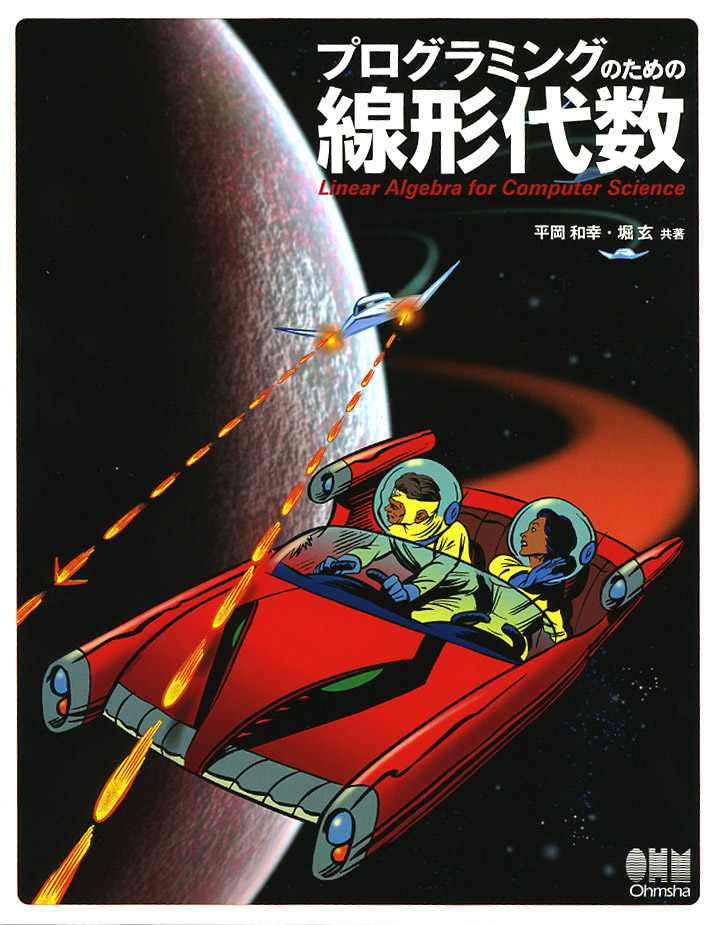
\includegraphics[width=.17\textwidth]{images/4-274-06578-2.jpg}     &
%    
\includegraphics[width=.17\textwidth]{images/978-4-274-06714-3.jpg} &
    
\includegraphics[width=.17\textwidth]{images/978-4-274-06876-8.jpg} &
    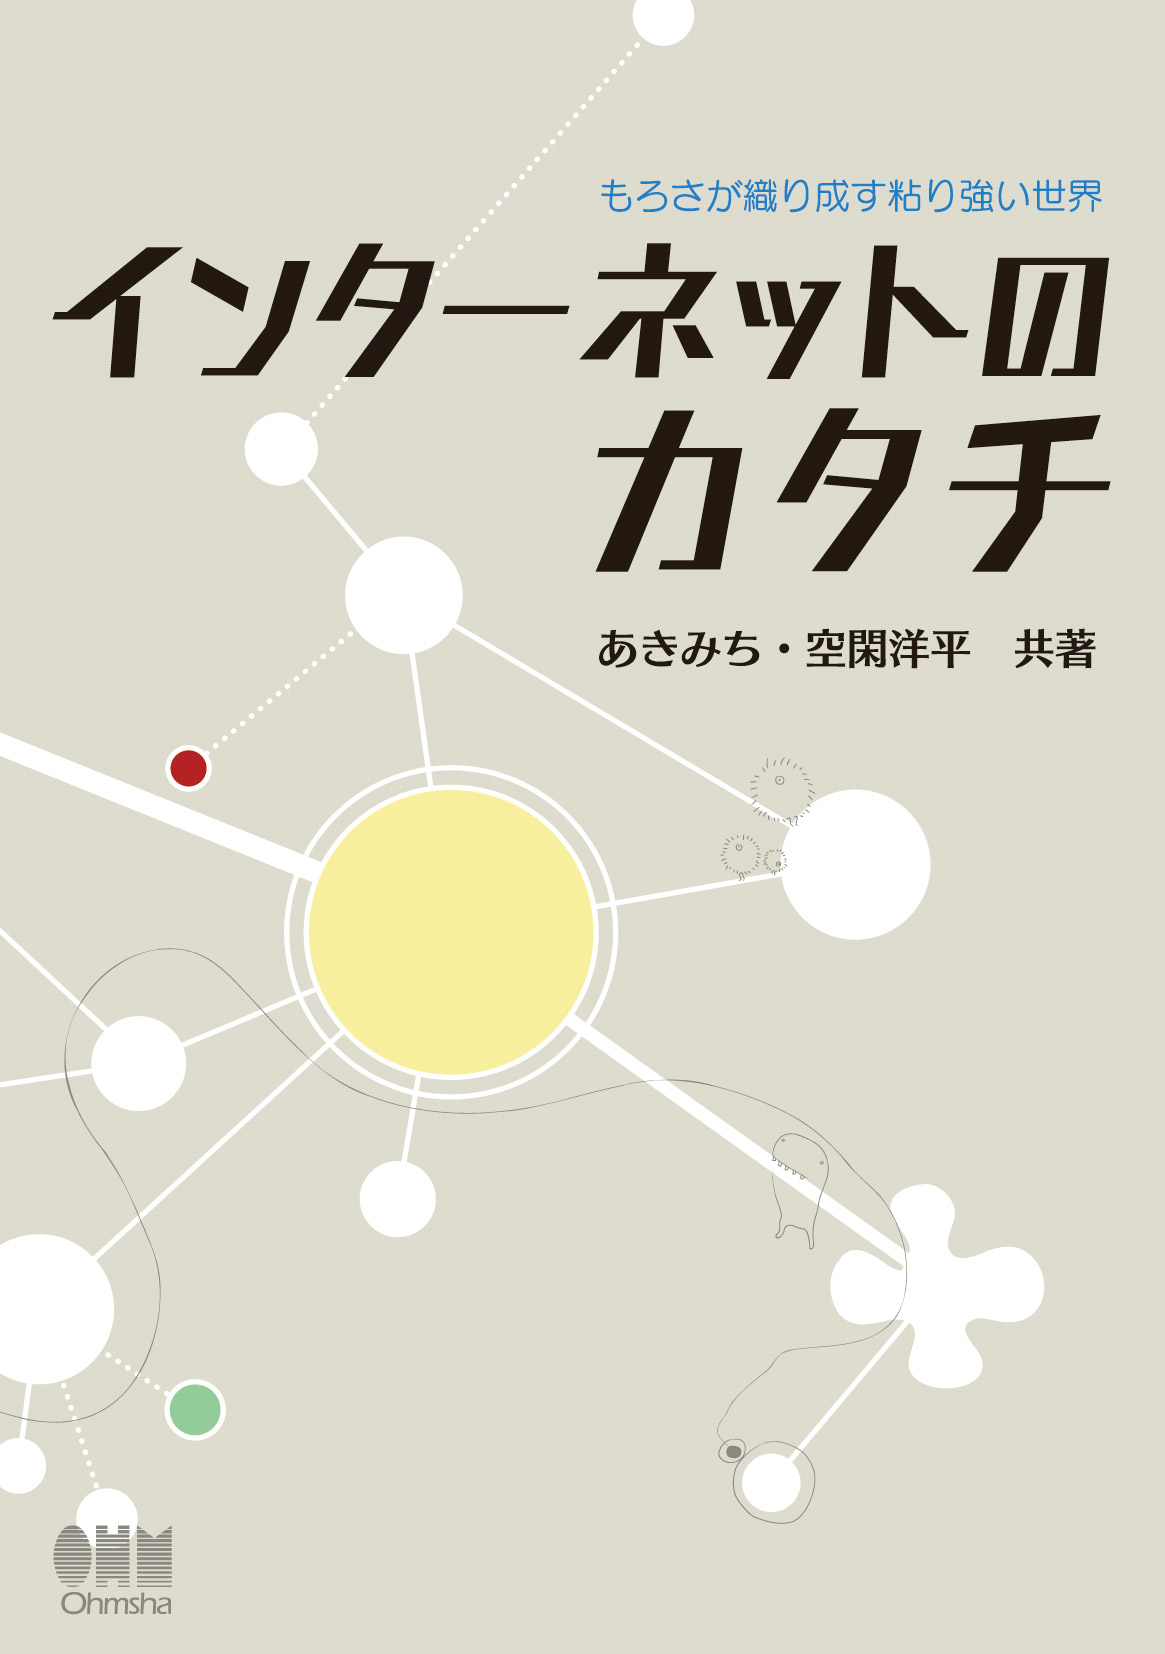
\includegraphics[width=.15\textwidth]{images/978-4-274-06824-9.jpg} &
    
\includegraphics[width=.15\textwidth]{images/978-4-274-06767-9.jpg} &
    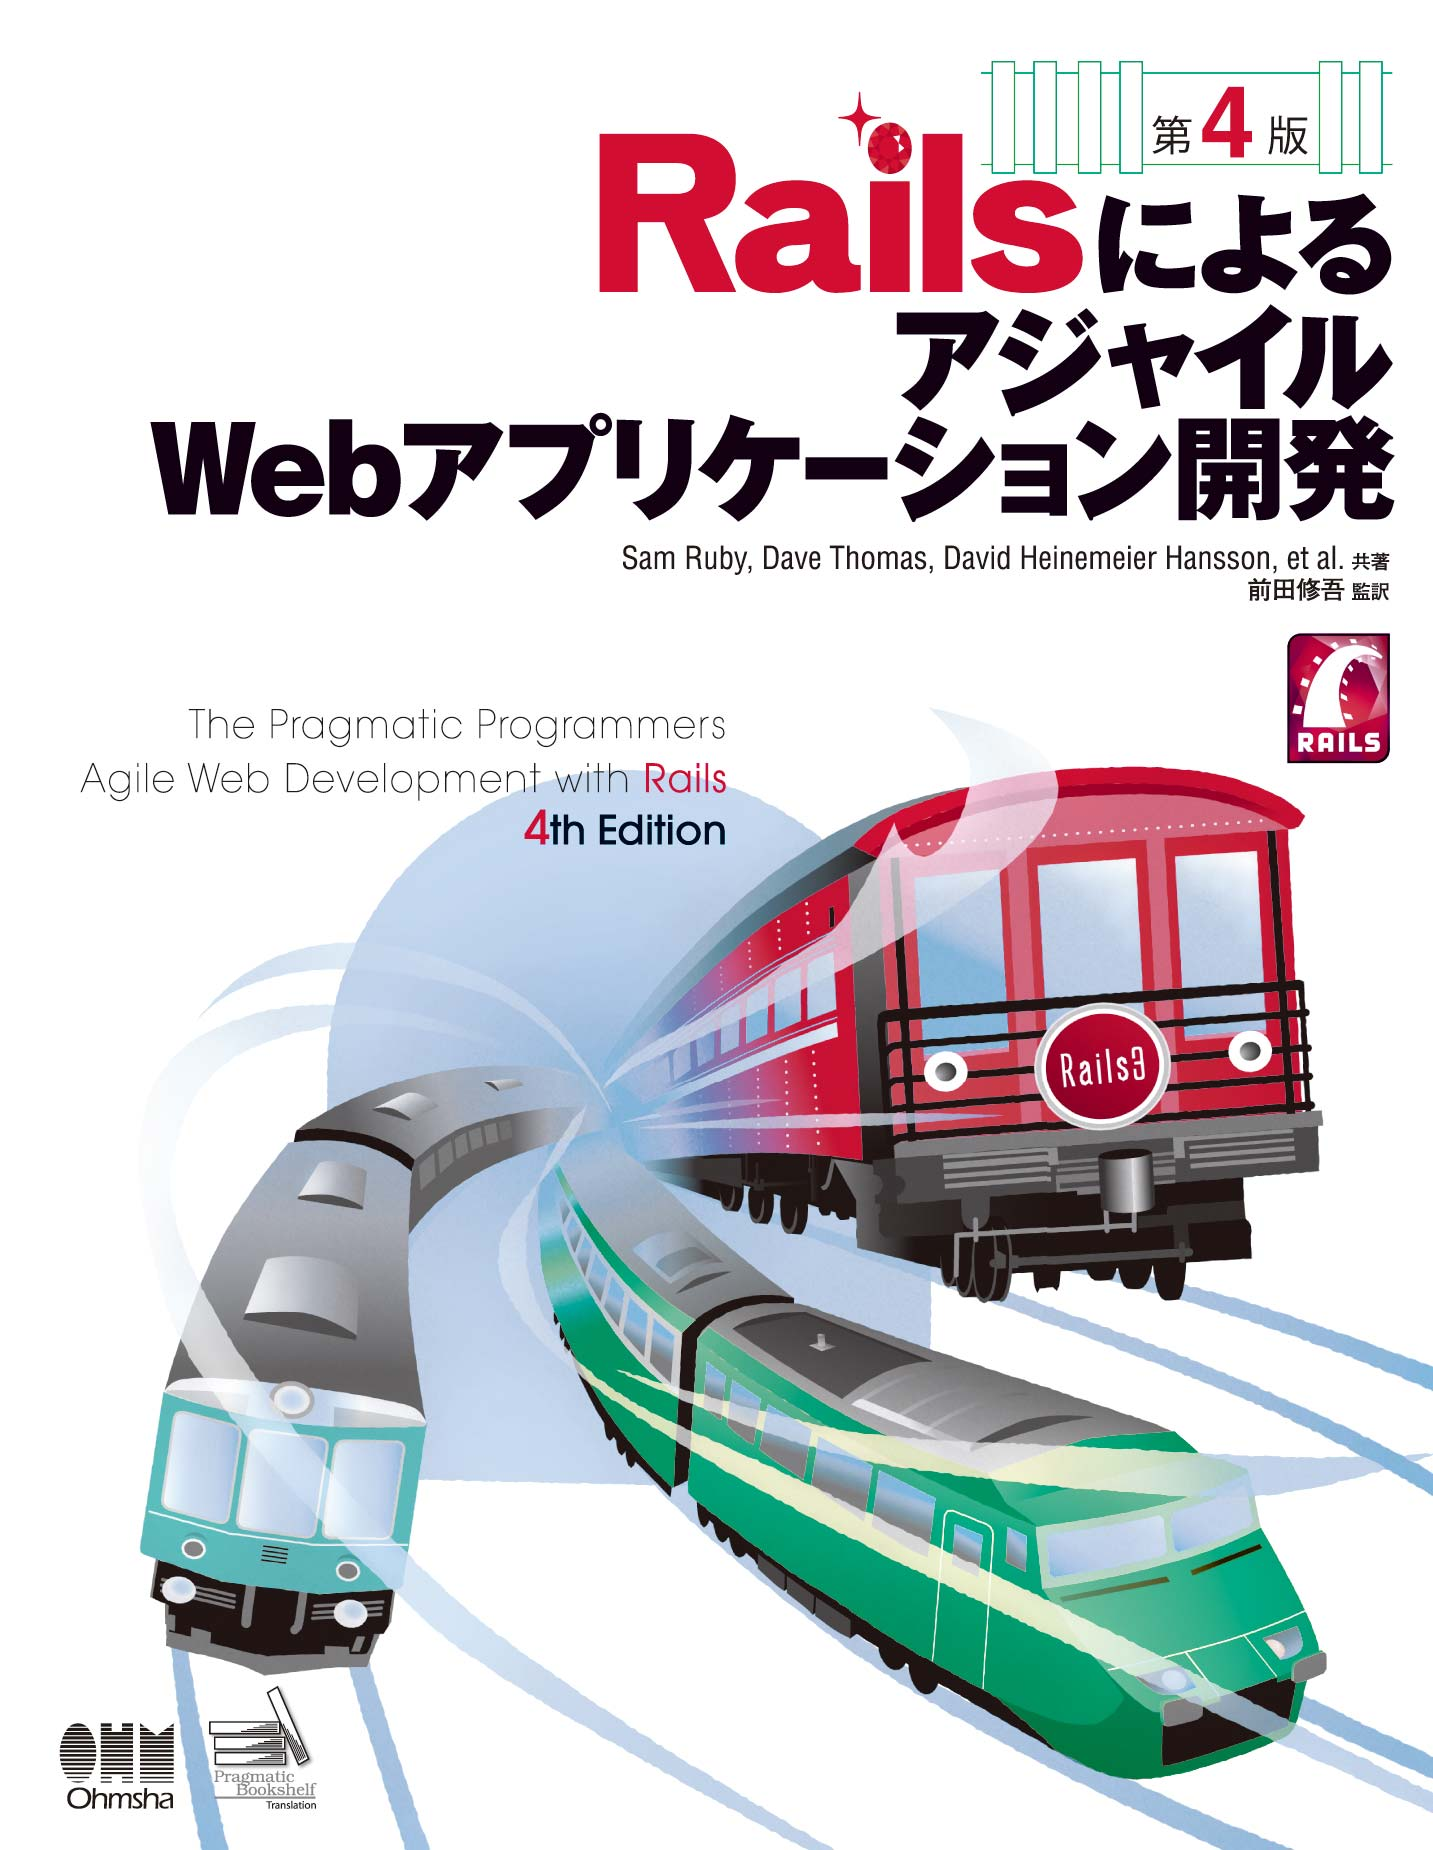
\includegraphics[width=.17\textwidth]{images/978-4-274-06866-9.jpg} \\
    
\includegraphics[width=.17\textwidth]{images/978-4-274-06944-4.jpg} &
    
\includegraphics[width=.17\textwidth]{images/978-4-274-06911-6.jpg} &
    
\includegraphics[width=.15\textwidth]{images/978-4-274-06885-0.jpg} &
    
\includegraphics[width=.15\textwidth]{images/978-4-274-06912-3.jpg} &
    
\includegraphics[width=.15\textwidth]{images/978-4-274-21762-3.jpg} 
  \end{tabular}
\end{frame}

\begin{frame}[t]{\inhibitglue 職務経歴書}
  \sffamily

  \begin{itemize}
    \item IT系の技術書を世に出す仕事
    \item 職務経歴書:{\footnotesize \url{http://note.golden-lucky.net/2015/09/blog-post.html}}
  \end{itemize}

\begin{tikzpicture}
  \node at (0,0){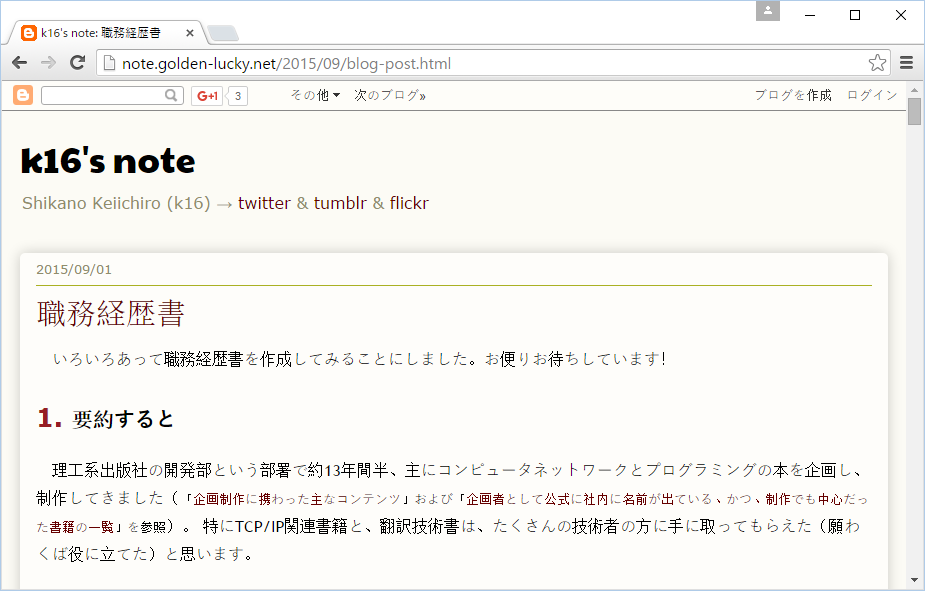
\includegraphics[width=.7\textwidth]{images/kereki1.png}};
\end{tikzpicture}

\end{frame}

\begin{frame}[t]{\inhibitglue 制作システムの開発}
  \sffamily

  \begin{itemize}
    \item IT系の技術書を世に出す仕事
    \item 職務経歴書:{\footnotesize \url{http://note.golden-lucky.net/2015/09/blog-post.html}}
  \end{itemize}

\begin{tikzpicture}
  \node at (0,0){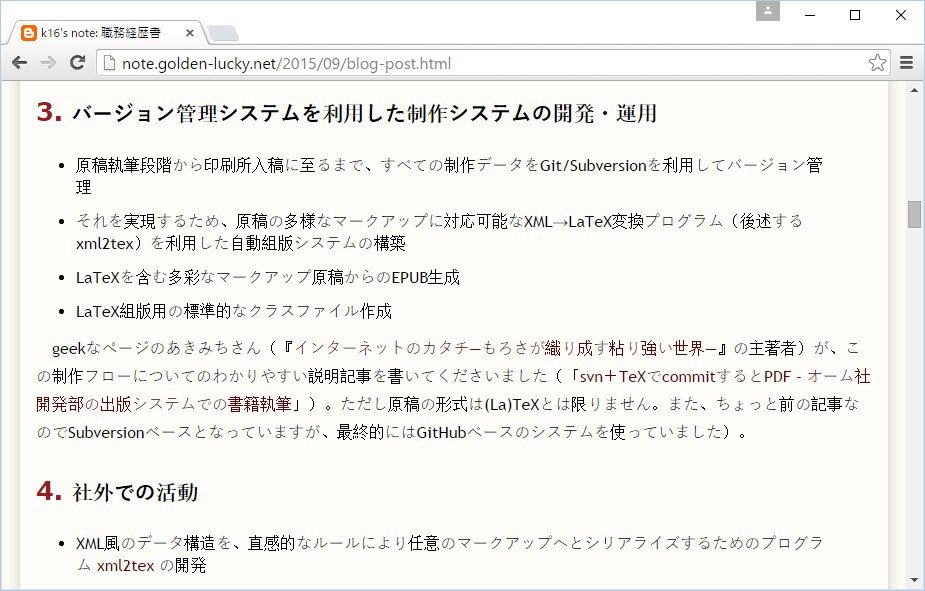
\includegraphics[width=.7\textwidth]{images/kereki2.png}};
  \pause;
  \node[notice={(-1,0.5)}, text width=4.5cm] at (0,-0.5) {自動組版システム?};
  \pause;
  \node[notice={(1,-1)}, text width=1.7cm] at (2,-2) {WTF?};
\end{tikzpicture}

\end{frame}

\begin{frame}[t]{\inhibitglue 版管理+自動組版システム}
  \sffamily

  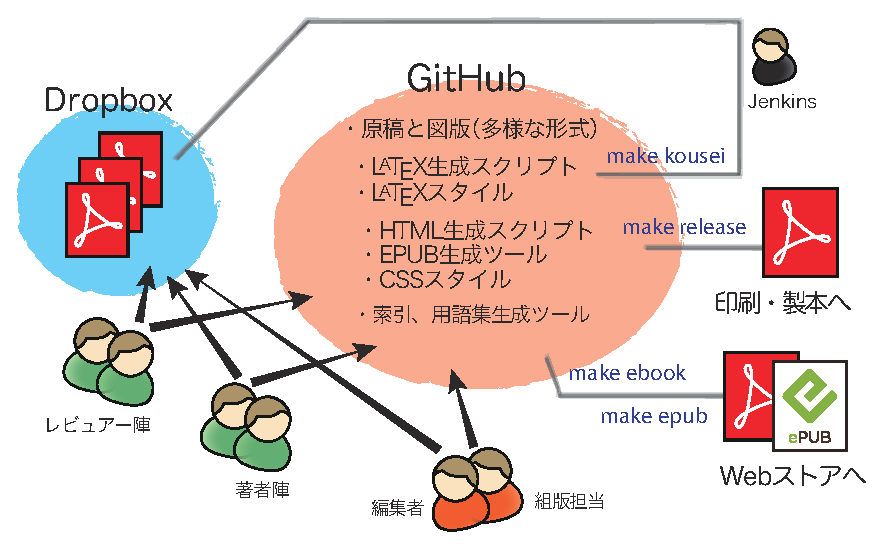
\includegraphics[width=1\textwidth]{images/vcs-centric.pdf}

\end{frame}

\begin{frame}[t]{\inhibitglue 版管理+自動組版イベント}
  \sffamily

\begin{tikzpicture}
  \node at (0,0){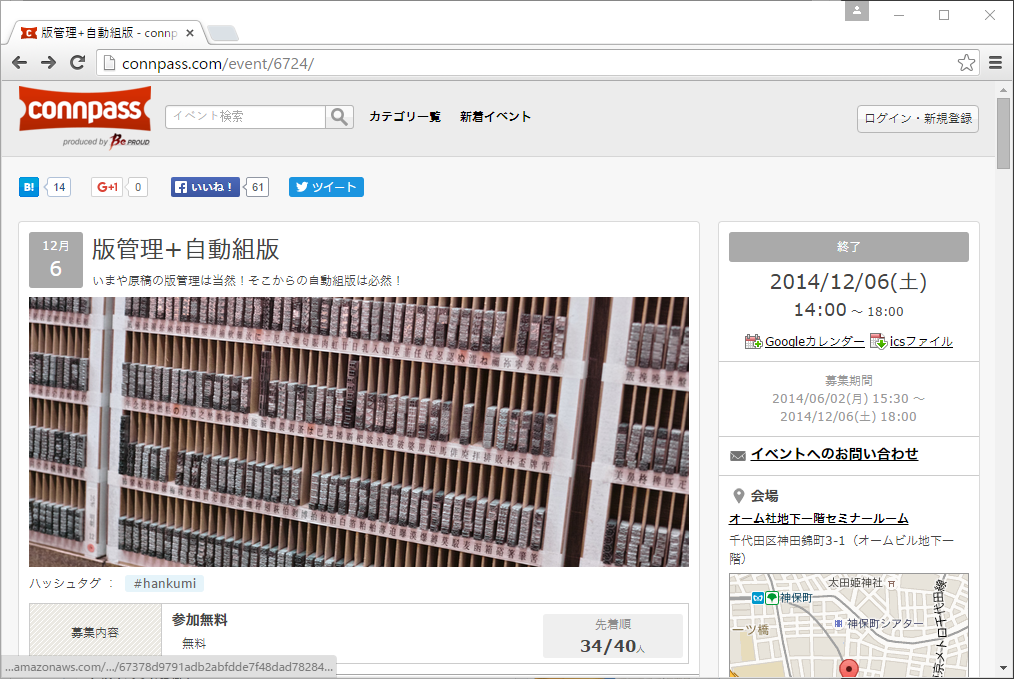
\includegraphics[width=.9\textwidth]{images/hankumi.png}};
  \pause;
  \node[notice={(-2.5,1)}, text width=4cm] at (-2,0) {いつかは第2回!};
\end{tikzpicture}

\end{frame}




\setbeamertemplate{background canvas}[vertical shading][bottom=white,top=kyara!15]
\setbeamercolor{frametitle}{bg=kyara, fg=white}
\setbeamercolor{structure}{fg=kyara}

\begin{frame}[plain]
\setlength{\textwidth}{115mm}
  \begin{center}
    \HUGE{34}{34}\color{kachi}\yasagoth
    ドキュメントシステムとは
  \end{center}
\end{frame}

%\begin{frame}[plain]
%  \HUGE{24}{34}\color{kachi}\yasagoth
%  \noindent ドキュメントシステムとは
%  
%  \begin{tcolorbox}\small\rmfamily
%  \HUGE{25}{32}
%  テキスト原稿を、人間が視覚的に読みやすくレイアウトする仕組み
%  \end{tcolorbox}
%\end{frame}


\def\software{\color{black}}
\def\book{\color{black}}
\def\markup{\color{black}}
\def\wysiwyg{\color{black}}
\def\historical{\color{black}}
\def\utility{\color{black}}
\def\formatter{\color{black}}
\def\cms{\color{black}}

\def\documentsystems{%
  \HUGE{10}{11}\vskip-\baselineskip
  \begin{columns}[t]
    \begin{column}{.28\textwidth}
    \begin{itemize}
      \item {\software POD}
      \item {\software Javadocなど}
      \item {\software WEB}
      \item {\software Sphinx}
%      \item {\software lhs2TeX}

      \item {\book Re:VIEW}
      \item {\book EWB}
      \item {\book CAS-UB}
      \item {\book Atlas}
      \item {\book Gitbook}
      \item {\book PressBooks}
%      \item {\book Leanpub}
      \item {\book Booktype}
      \item {\book IGP digital publisher}
      \item {\book BCCKS}
      \item {\book でんでんコンバータ}
%      \item {\book ideotype}
    \end{itemize}
    \end{column}
    \begin{column}{.37\textwidth}
    \begin{itemize}
      \item {\markup Markdown}
      \item {\markup Wiki記法}
      \item {\markup reStructuredText}
      \item {\markup RD、RDoc}
      \item {\markup AsciiDoc}
      \item {\markup HTMLBook}
      \item {\markup DocBook}
      \item {\markup DITA、JATS}
      \item {\markup \LaTeX とか}

      \item {\utility Docutils}
      \item {\utility Calibre}
      \item {\utility Pandoc}

      \item {\wysiwyg Word(MS Office)}
      \item {\wysiwyg Writer(LibreOffice)}
      \item {\wysiwyg Adobe InDesign}
      \item {\wysiwyg Adobe FrameMaker}
%      \item {\wysiwyg Scribus}
    \end{itemize}
    \end{column}
    \begin{column}{.31\textwidth}
    \begin{itemize}
      \item {\formatter AH Formatter}
      \item {\formatter Prince}
      \item {\formatter Apache FOP}

      \item {\formatter Vivliostyle}

      \item {\formatter \TeX エンジン}
      
      \item {\formatter ブラウザエンジン}
      \item {\formatter CSS Books}

      \item {\formatter cl-typesetting + cl-pdf}

      \item {\cms Wikipedia}
      \item {\cms WordPress}

      \item {\historical Scribe}
      \item {\historical roff系}
      \item {\historical Setext}
      \item {\historical Jade(SGML+DSSSL)}
    \end{itemize}
    \end{column}
  \end{columns}
}

\begin{frame}[t]{\inhibitglue 思いつくキーワードを挙げてみた}
  \sffamily
  \documentsystems
  
\end{frame}

\begin{frame}[t]{\inhibitglue 歴史遺産}
  \sffamily
  \def\historical{\color{shozyohi}}
  \documentsystems
\end{frame}
  \def\historical{\color{torinoko}}

\begin{frame}[t]{\inhibitglue CMS}
  \sffamily
  \def\cms{\color{shozyohi}}
  \documentsystems
\end{frame}

  \def\cms{\color{torinoko}}

\begin{frame}[t]{\inhibitglue DTPソフト}
  \sffamily
  \def\wysiwyg{\color{shozyohi}}
  \documentsystems
\end{frame}

  \def\wysiwyg{\color{torinoko}}

\begin{frame}[t]{\inhibitglue 入力{\footnotesize ( マークアップ、XMLアプリケーションなど)}}
  \sffamily
  \def\markup{\color{moegi}}
  \documentsystems
\end{frame}

\begin{frame}[t]{\inhibitglue 出力{\footnotesize (フォーマッタ、スタイルシートなど)}}
  \sffamily
  \def\markup{\color{black}}
  \def\utility{\color{black}}
  \def\formatter{\color{ruri}}
  \def\wysiwyg{\color{ruri}}
  \documentsystems
\end{frame}

\begin{frame}[t]{\inhibitglue 汎用変換ツール}
  \sffamily
  \def\book{\color{black}}
  \def\markup{\color{black}}
  \def\formatter{\color{black}}
  \def\utility{\color{black!20!ginshu}}
  \documentsystems
\end{frame}

  \def\markup{\color{moegi}}
  \def\formatter{\color{ruri}}
  \def\wysiwyg{\color{ruri}}
  \def\utility{\color{ginshu}}

\begin{frame}[t]{\inhibitglue ソフトウェアのドキュメント向け}
  \sffamily

  \def\software{\color{shozyohi}}
  
  \documentsystems
\end{frame}

\begin{frame}[t]{\inhibitglue 書籍向け(特化)}
  \sffamily
  \def\software{\color{black}}
  \def\book{\color{shozyohi}}
  \documentsystems
\end{frame}

\begin{frame}[t]{\inhibitglue ドキュメントシステムを特徴づける要素}
  \sffamily

  \begin{itemize}
    \item 入力方法(マークアップ方法)\\
      \begin{itemize}
        \item レイアウトの指定方法
        \item 構造の指定方法
        \item メタ情報の指定方法
      \end{itemize}
    \item 出力の用途(品質)\\
      \begin{itemize}
        \item APIマニュアル
        \item Webサイト
        \item 単一記事
        \item 電子書籍
        \item 紙書籍
      \end{itemize}
  \end{itemize}

\end{frame}




\setbeamertemplate{background canvas}[vertical shading][bottom=white,top=kachi!15]
\setbeamercolor{frametitle}{bg=kachi, fg=white}
\setbeamercolor{structure}{fg=kachi}

\begin{frame}[plain]
  \begin{center}
    \HUGE{34}{34}\color{kachi}\yasagoth
    マークアップから\\ 考える
  \end{center}
\end{frame}

\tikzstyle{every node}=[font=\scriptsize]
\tikzset{
  >=stealth',
  fmt/.style  = { draw, fill=yamabuki, black, rounded corners, text centered},
  suc/.style = { ->, thick, shorten <=-2pt, shorten >=-2pt},
  sim/.style = {ruri, ->, decorate, decoration={snake, pre length=2pt, post length=2pt, amplitude=2pt}, >=stealth, thick, shorten <=-2pt, shorten >=-2pt}
}
\def\historyofmarkup{%
  \begin{tikzpicture}[remember picture,overlay]
  \node[fmt] (text90) at (0.75,0.25) {Text90};
  \node[fmt, right=0.3cm of text90] (runoff) {RUNOFF};
  \node[fmt, right=0.5cm of runoff] (troff) {TRoff};
  \node[right=0.3cm of runoff] (dummy0) {};
  \node[fmt, below=0.05cm of dummy0] (eqn) {EQN};

  \node[right=0.3cm of text90] (dummy1) {};
  \node[fmt, below=0.5cm of dummy1] (tex) {\TeX};

  \node[fmt, below=0.5cm of tex] (scribe) {Scribe};
  \node[right=2cm of scribe] (dummy2) {};
  \node[fmt, above=0.25cm of dummy2] (latex) {\LaTeX};

  \node[fmt, below=0.5cm of scribe] (gml) {IBM GML};
  \node[fmt, right=0.25cm of gml] (sgml) {SGML};
  \node[right=1cm of sgml] (dummy3) {};
  \node[fmt, above=0.25cm of dummy3] (html) {HTML};
  \node[fmt, below=-0.25cm of dummy3] (xml) {XML};
  \node[fmt, right=1.5cm of xml] (asciidoc) {AsciiDoc};

  \node[fmt, below=3cm of sgml] (ewb) {EWB};
  \node[fmt, right=4.5cm of ewb] (review) {Re:VIEW};

  \node[below=5cm of text90] (dummy4) {};
  \node[fmt, right=0cm of dummy4, text width=3em] (web) {文芸的プログラミング};
  \node[fmt, right=0.25cm of web, text width=3.5em] (swd) {ソフトウェアドキュメント};
  \node[fmt, right=0.25cm of swd] (pod) {pod};
  \node[fmt, below=0.25cm of xml] (setext) {setext};
  \node[fmt, right=0.5cm of pod] (rest) {reST};
  \node[fmt, right=0.5cm of rest] (md) {Markdown};
  \node[fmt, below=0.25cm of rest] (rd) {RD};

  \node[fmt, right=0.5cm of html] (wiki) {Wiki記法};
  \node[right=3.5cm of html] (dummy5) {};
  \node[fmt, above=0.75cm of dummy5] (htmlbook) {HTMLBook};

  \node[right=of md] (dummy6) {};
  \node[above=0cm of dummy6] (dummy7) {};
  \node[below=0cm of dummy6] (dummy8) {};

  \draw[suc] (text90) to (runoff);
  \draw[suc] (runoff) to (troff);
  \draw[suc] (gml) to (sgml);
  \draw[suc] (sgml) to (xml);
  \draw[sim] (sgml) to (html);
  \draw[suc] (scribe) to (sgml);
  \draw[suc] (scribe) to (html);
  \draw[suc] (scribe) to (latex);
  \draw[sim] (html) to (wiki);
  \draw[sim] (html) to (htmlbook.west);
  \draw[sim] (xml) to (asciidoc);
  \draw[suc, <->] (eqn) to (tex);
  \draw[suc] (tex) to (latex);
  \draw[suc] (web) to (swd);
  \draw[suc] (swd) to (pod);
  \draw[suc] (pod) to (rest);
  \draw[suc] (pod) to (rd);
%  \draw[sim] (sgml) to (setext);
  \draw[suc] (setext) to (rest);
  \draw[suc] (setext) to (md);
  \draw[sim] (html) to (md);
  \draw[suc] (rest) to (md);
  \draw[suc] (ewb) to (review);
  \draw[suc] (rd) to (review);

  \draw[suc] (md) to (dummy6);
  \draw[suc] (md) to (dummy7);
  \draw[suc] (md) to (dummy8);
  \end{tikzpicture}
}

\begin{frame}[t]{\inhibitglue 入力フォーマットの起源と変遷}
  \sffamily
  \historyofmarkup
\end{frame}

\begin{frame}[t]{\inhibitglue 入力フォーマットの起源と変遷$^{\ \text{[要出典]}}$}
  \sffamily
  \historyofmarkup
\end{frame}

\begin{frame}[t]{\inhibitglue 入力フォーマットの起源と変遷$^{\ \text{[要出典]}}$}
  \sffamily
  \historyofmarkup
  \begin{tikzpicture}[remember picture,overlay]
  \node[notice={(0.75,0.15)}, font=\small, text width=4cm, text centered] at (2,-1.5) {ターゲット向けの出力指示をコマンドとしてテキスト中に挿入};
  \node[notice={(2,0.15)}, font=\small, text width=4cm, text centered] at (2,-1.5) {ターゲット向けの出力指示をコマンドとしてテキスト中に挿入};
  \node[notice={(4,0.15)}, font=\small, text width=4cm, text centered] at (2,-1.5) {ターゲット向けの出力指示をコマンドとしてテキスト中に挿入};
  \pause;
  \node[notice={(3.5,-6.25)}, font=\small, text width=2cm, minimum height=1cm, text centered] at (4,-5) {これも?};
  \end{tikzpicture}

\end{frame}

\begin{frame}[t]{\inhibitglue 入力フォーマットの起源と変遷$^{\ \text{[要出典]}}$}
  \sffamily
  \historyofmarkup
  \begin{tikzpicture}[remember picture,overlay]
  \node[notice={(2.25,-2.85)}, font=\small, text width=3cm, minimum height=2cm, text centered] at (4.75,-2.5) {ターゲットによらない高レベルな記述を意識};
  \node[notice={(3.75,-0.35)}, font=\small, text width=3cm, minimum height=2cm, text centered] at (4.75,-2.5) {ターゲットによらない高レベルな記述を意識};
  \end{tikzpicture}

\end{frame}

\begin{frame}[t]{\inhibitglue 入力フォーマットの起源と変遷$^{\ \text{[要出典]}}$}
  \sffamily
  \historyofmarkup
  \begin{tikzpicture}[remember picture,overlay]
  \node[notice={(1.65,-2)}, font=\small, text width=3cm, minimum height=2cm, text centered] at (1.5,-3.5) {構造と表現の分離という概念の発明};
  \end{tikzpicture}

\end{frame}

\begin{frame}[t]{\inhibitglue 入力フォーマットの起源と変遷$^{\ \text{[要出典]}}$}
  \sffamily
  \historyofmarkup
  \begin{tikzpicture}[remember picture,overlay]
    \draw[thick] (7,0.55) rectangle (11.25,-0.25);
    \draw[sim] (7.5,0.15) to (8.5,0.15);
    \node[text width=2cm,black,font=\scriptsize] at (10,0.15) {特定ターゲット向けに簡素化};
    \pause;
    \node[notice={(10.25,-0.15)}, font=\small, text width=2.5cm, minimum height=1.5cm, text centered] at (10,-1.65) {先祖返り?};

  \end{tikzpicture}

\end{frame}


\begin{frame}[t]{\inhibitglue 入力フォーマットの指向性}
  \sffamily
  \noindent\hspace*{-2em}
  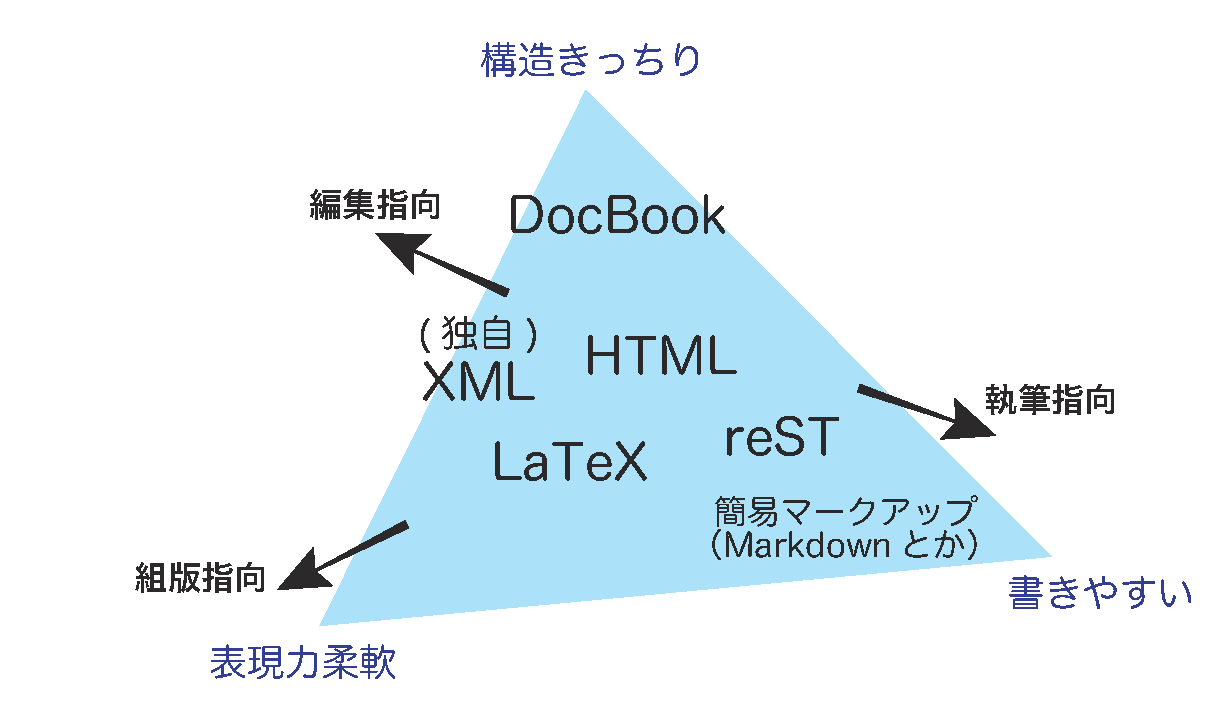
\includegraphics[width=\textwidth]{images/docsystems1.pdf}

\end{frame}





\setbeamertemplate{background canvas}[vertical shading][bottom=white,top=yamabuki!15]
\setbeamercolor{frametitle}{bg=yamabuki, fg=black}
\setbeamercolor{structure}{fg=yamabuki}

\begin{frame}[plain]
  \begin{center}
    \HUGE{34}{34}\color{black}\yasagoth
    出力の用途から\\ 考える
  \end{center}
\end{frame}

\begin{frame}[containsverbatim, t]{\inhibitglue Yes/Noチャート(異論は認める)}
  \sffamily
  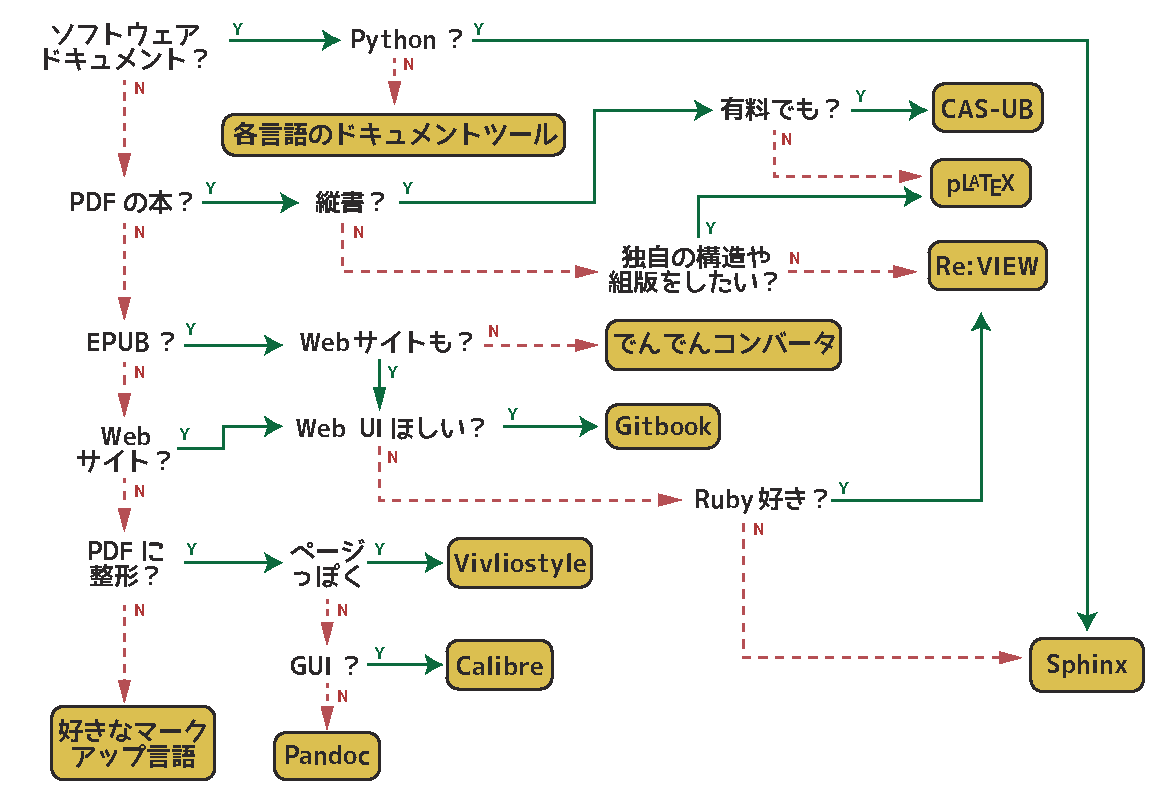
\includegraphics[width=.95\textwidth]{images/ynchart.pdf}
\end{frame}

\begin{frame}[containsverbatim, t]{\inhibitglue Sphinx}
  \sffamily
  
  \begin{itemize}
    \item ドキュメントをPDFでもEPUBでもHTMLでも出力したいといった用途に幅広く便利
    \item 特に、Pythonプログラムのドキュメントならこれ一択
    \item 構文などの拡張性は高い。既存の便利なエクステンションも豊富
    \item 紙書籍向けサポートは弱い
    \item \url{http://sphinx-doc.org/}(\url{http://sphinx-users.jp/})
  \end{itemize}

\end{frame}

\begin{frame}[containsverbatim, t]{\inhibitglue Re:VIEW}
  \sffamily
  
  \begin{itemize}
    \item 横書きの技術書(紙書籍向けPDF、電子書籍向けPDF、EPUB)が作りやすい
    \item 構文などの拡張性は高い
    \item 見た目をデフォルト以外にしたければ出力(LaTeX、CSS、InDesign)の知識が不可欠
    \item \url{https://github.com/kmuto/review/wiki}
  \end{itemize}

\end{frame}

%\begin{frame}[containsverbatim, t]{\inhibitglue EWB}
%  \sffamily
%  
%  \begin{itemize}
%    \item LaTeXっぽいシンタックスでテキストにレイアウト指示を入れる
%    \item アスキードワンゴで出版するなら、最有力
%  \end{itemize}
%
%\end{frame}

\begin{frame}[containsverbatim, t]{\inhibitglue Gitbook}
  \sffamily
  
  \begin{itemize}
    \item 技術書がGitHubとMarkdown(AsciiDomも可)で書ける。Web UIもある
    \item 構文の拡張性はないが、ある程度のスタイルは定義可能。いくつかプラグインもある
    \item PDF出力がひどい(CalibreのPDFエンジン)
    \item \url{https://www.gitbook.com}(\url{https://github.com/GitbookIO/gitbook})
  \end{itemize}

\end{frame}

\begin{frame}[containsverbatim, t]{\inhibitglue CAS-UB}
  \sffamily
  
  \begin{itemize}
    \item 縦書きを含む日本語の本(紙書籍向けPDF、電子書籍向けPDF、EPUB)が作れて、売れる
    \item 構文の拡張性はないが、ある程度のスタイルは定義可能
    \item Webブラウザでの編集が基本。1カ月の無償期間を超えると有償
    \item \url{http://www.cas-ub.com/index.php}
    \item (PressBooks、Booktype、Lean Book、Atlasなど、ほかにも同様の書籍執筆Webサービスはある)
  \end{itemize}

\end{frame}

%\begin{frame}[containsverbatim, t]{\inhibitglue PressBooks}
%  \sffamily
%  
%  \begin{itemize}
%    \item まともな本が作れて売れる
%    \item HTMLとCSSで書ける
%    \item PDFはPrinceで生成
%    \item Webブラウザでの編集が基本。課金しないと全ページに透かしが入る。日本語はNotoSans一択
%  \end{itemize}
%
%\end{frame}

%\begin{frame}[containsverbatim, t]{\inhibitglue Booktype}
%  \sffamily
%  
%  \begin{itemize}
%    \item 本が作れる。
%    \item HTMLとCSSで書ける
%    \item PDFはmPDF(PHPのネイティブなPDFエンジンであるFPDFの拡張)で生成
%    \item 日本語は文字化け
%  \end{itemize}
%
%\end{frame}
%
%\begin{frame}[containsverbatim, t]{\inhibitglue Atlas}
%  \sffamily
%  
%  \begin{itemize}
%    \item 米O'Reillyの著者用プラットフォーム
%    \item 入力はAsciiBooksとHTMLBooksで、出力はAH Formatterらしい
%    \item O'Reillyの著者にならないと使えない
%  \end{itemize}
%
%\end{frame}

\begin{frame}[containsverbatim, t]{\inhibitglue でんでんコンバーター}
  \sffamily
  
  \begin{itemize}
    \item 縦書きを含む日本語のEPUBが作れる
    \item 構文はMarkdownの独自拡張だが、HTMLの埋め込みはできる
    \item EPUBのみを生成するなら特に不満はないような?
    \item \url{http://conv.denshochan.com/}
  \end{itemize}

\end{frame}

%\begin{frame}[containsverbatim, t]{\inhibitglue BCCKS}
%  \sffamily
%  
%  \begin{itemize}
%    \item 縦書きを含め、まともな本(EPUBと紙)が作れて売れる
%    \item Wiki記法
%    \item 基本的にはEPUB出版用のサービスだが、オンデマンド用のPDF生成サービスがある
%    \item PDFがほしい場合には使えない
%  \end{itemize}
%
%\end{frame}


\begin{frame}[containsverbatim, t]{\inhibitglue Vivliostyle}
  \sffamily
  
  \begin{itemize}
    \item CSS組版エンジン
    \item Webブラウザで本のようなページが動的にレンダリングできる
    \item Webページ用のCSSからPDFが作れるわけではない
    \item \url{http://vivliostyle.com/ja/}
  \end{itemize}

\end{frame}

%\begin{frame}[containsverbatim, t]{\inhibitglue xml2tex}
%  \sffamily
%  
%  \begin{itemize}
%    \item XMLのシンタックスをLaTeXのシンタックスに対応づけるルールベース変換器
%    \item Gauche製
%    \item LaTeXに限らず、MarkdownやRe:VIEWフォーマットなどへの変換ルールも定義可能
%  \end{itemize}
%
%\end{frame}

\begin{frame}[containsverbatim, t]{\inhibitglue Pandoc}
  \sffamily
  
  \begin{itemize}
    \item さまざまなフォーマットを変換できる。似たようなツールはほかにもあるけど(kramdownとか)、対応フォーマット数が多く、しかも増えている
    \item Haskell製
    \item 基本的にはMarkdownを他の書式に変換するためのツールだと割り切ったほうが良い
    \item \url{http://pandoc.org/}
  \end{itemize}

\end{frame}

\begin{frame}[containsverbatim, t]{\inhibitglue Calibre}
  \sffamily
  
  \begin{itemize}
    \item 電子書籍の統合開発環境。なんでもできる。コマンド(\texttt{ebook-convert})もある
    \item Python製
    \item EPUB3には未対応
    \item \url{http://calibre-ebook.com/}
  \end{itemize}

\end{frame}



\setbeamertemplate{background canvas}[vertical shading][bottom=white,top=miru!15]
\setbeamercolor{frametitle}{bg=miru, fg=white}
\setbeamercolor{structure}{fg=miru}

\begin{frame}[plain]
  \begin{center}
    \HUGE{34}{34}\color{miru}\yasagoth
    結論
  \end{center}
\end{frame}

\begin{frame}[containsverbatim, t]{\inhibitglue ドキュメントシステムの選び方}
  \sffamily
  
  \begin{itemize}
    \item ドキュメントシステムとは、テキスト本体にマークアップされた情報を使って、人間が視覚的に読みやすいレイアウトを生成する仕組みである
  \end{itemize}
  
  \begin{itemize}
    \item シンプルなマークアップは、ターゲットを決め打ちした結果かもしれない
    \item そもそも視覚的な読みやすさだけが目標でいいのか(構造を読み取るデバイスは肉眼とは限らない)
    \item その意味では、XMLは強い
  \end{itemize}

  \begin{itemize}
    \item なんでも好きなものを選べる状況なら、書きやすいマークアップ(あるいはWeb UI)があるとか、必要なターゲット向けに素敵なテンプレートがあるとか、そんな基準でいいのかもしれない
  \end{itemize}

\end{frame}




\begin{frame}[containsverbatim, t]{\inhibitglue 参考資料、URL}
  \sffamily
  \footnotesize

  \begin{itemize}
    \item Martin Bryan著, 山崎俊一監訳 ``SGML入門''(アスキー出版局, 1991)
    \item Brian Reid ``Scribe: A Document Specification Language and its Compiler''(Doctor Thesis, 1980)
    \item Leslie Lamport著, Edgar Cooke・倉沢良一監訳 ``文書処理システム\LaTeX ''(アスキー出版局, 1990)
    \item O'Reilly Media ``Using Web Standards in Print and Digital Book Workflows'' \url{http://www.w3.org/2012/12/global-publisher/slides/Day1/P0-witwer_adam.pdf}
  \end{itemize}

  \begin{itemize}
    \item pod:\url{http://perldoc.perl.org/perlpod.html}
    \item AsciiDoc:\url{http://www.methods.co.nz/asciidoc/}
    \item HTMLBook:\url{http://jagat-xml-publishing-study-group.github.io/HTMLBook-JA/}
    \item Philosophy of Markdown:\url{https://daringfireball.net/projects/markdown/syntax#philosophy}
  \end{itemize}

\end{frame}




\end{document}
